\chapter{OpenMP}
Definiamo un \textbf{processo} come una sequenza indipendente di istruzioni e l'insieme di risorse necessarie alla sua esecuzione. Questi, infatti, devono accedere a uno spazio di memoria protetto e a delle risorse del sistema.

Possono esistere più processi in esecuzione che eseguono lo stesso programma in maniera del tutto indipendente che possiedono, quindi, diverse risorse del sistema indipendenti li uni dalle altre.

\begin{figure}[H]
    \centering
    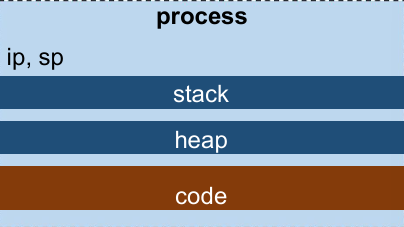
\includegraphics[width=0.5\linewidth]{Images/cap_6/processo.png}
\end{figure}

Al contrario, un \textbf{thread} è un'istanza indipendente di esecuzione di un codice all'\textbf{interno di un processo}. Possono esserci, dunque, più thread in esecuzione sullo stesso processo. Ognuno di questi, condivide lo stesso codice, lo stesso spazio di indirizzamento e le stesse risorse del processo padre. Siamo in un modello a \textbf{memoria condivisa} in cui ogni unità di elaborazione (i thread) condivide la stessa memoria ma con un piccolo spazio \textbf{privato}, come in un'architettura NUMA. 
\begin{figure}[H]
    \centering
    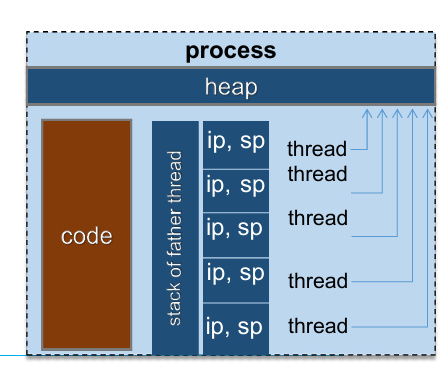
\includegraphics[width=0.5\linewidth]{Images/cap_6/processo_thread.png}
\end{figure}

In generale, generare thread all’interno di un processo è molto meno costoso che creare processi.

A seconda dell'architettura hardware, si utilizzano paradigmi software differenti.

\begin{itemize}
    \item \textbf{Shared-Memory (es. OpenMP)}: Un singolo processo univoco genera un certo numero di thread. Poiché esiste uno spazio di memoria univoco (l'Heap del processo), la comunicazione tra thread avviene in modo \textit{implicito} leggendo e scrivendo le stesse variabili in memoria.
    \item \textbf{Distributed-Memory (es. MPI)}: Vengono creati $N$ processi distinti, ognuno con la propria copia del codice e il proprio spazio di memoria privato e isolato. Un processo non può fisicamente accedere alla memoria di un altro. La comunicazione deve avvenire obbligatoriamente in modo \textit{esplicito} tramite lo scambio di messaggi sulla rete.
\end{itemize}

\section{Cosa è OpenMP}
OpenMP (Open specifications for MultiProcessing) è un'API standard per la programmazione parallela a memoria condivisa. 
Consente di scrivere programmi multithread con un comportamento standard attraverso l'utilizzo di un set di direttive del compilatore da inserire nel codice sorgente. OpenMP permette di parallelizzare il codice sia suddividendo automaticamente piccoli lavori (come le iterazioni di un ciclo), sia assegnando esplicitamente compiti più grandi ai singoli thread.

\noindent
OpenMP è composto da 3 componenti:
\begin{enumerate}
    \item \textbf{Direttive del Compilatore}: In C/C++ assumono la forma di \texttt{\#pragma} e forniscono indicazioni su come gestire i thread.
    \item \textbf{Librerie di Runtime}: Funzioni richiamabili dal codice (es. per sapere quanti thread stanno lavorando).
    \item \textbf{Variabili d'Ambiente}: Parametri impostati dall'utente a livello di sistema operativo (es. per definire quanti thread generare o per gestire l'affinità core-memoria).
\end{enumerate}

I vantaggi di un approccio basato sulle direttive sono:

\begin{itemize}
    \item \textbf{Astrazione}: Le sottigliezze di pthread e gli aspetti specifici dell'hardware sono nascosti. È possibile concentrarsi sui dati e sul flusso di lavoro molto più facilmente.
    \item \textbf{Efficienza}: La curva di apprendimento per ottenere risultati ragionevoli è molto più semplice. La progettazione del codice è più semplice, il rapporto risultato/sforzo è favorevole rispetto a pthread.
    \item \textbf{Approccio incrementale}: Non è necessario riscrivere l'intero codice. Si inizia concentrandosi solo su alcune sezioni, seguendo i suggerimenti del profiling.
    \item \textbf{Portabilità}: Il compilatore si occuperà di questo per noi. È comunque necessario sviluppare una progettazione in grado di adattarsi a diverse topologie.
    \item \textbf{Un'unica fonte}: Attraverso la compilazione condizionale, le versioni seriali e parallele possono coesistere facilmente.
\end{itemize}

\section{Modello Fork-Join} 
OpenMP basa il suo funzionamento sul modello \textbf{Fork-Join}. 
Il programma inizia l'esecuzione come un normale programma sequenziale guidato da un \textbf{singolo thread master}.
\begin{itemize}
    \item \textbf{Fork}: Quando il thread master incontra una direttiva specifica (una regione parallela), genera un \textit{team di thread} figli per eseguire il lavoro in parallelo. Il master sospende la sua attività singola e si unisce al pool lavorando come "thread 0".
    \item \textbf{Join}: Al termine della regione parallela, i thread si sincronizzano. I thread figli terminano (o si mettono in pausa) e il solo thread master riprende l'esecuzione seriale del codice.
\end{itemize}

Il modello offre flessibilità nella gestione delle risorse, ma presenta vincoli stringenti riguardo alla struttura del codice:
\begin{itemize}
    \item \textbf{Dipendenze nei Loop}: Le dipendenze "trasportate" dai cicli (quando un'iterazione ha bisogno del risultato della precedente) rappresentano il principale ostacolo all'accelerazione parallela.
    \item \textbf{Parallelismo Annidato (Nested)}: È esplicitamente consentito creare regioni parallele all'interno di altre regioni parallele.
    \item \textbf{Modifica Dinamica}: Il numero di thread non è necessariamente fisso ma può essere modificato dinamicamente prima di entrare in una nuova regione parallela.
\end{itemize}
\subsection{Direttive}
Le direttive OpenMP si applicano a \textbf{blocchi di codice strutturati}, ovvero blocchi che hanno un singolo punto di ingresso e un singolo punto di uscita, senza istruzioni di salto (branch) incontrollati al loro interno.
La direttiva principale per avviare il parallelismo è:
\begin{verbatim}
#pragma omp parallel{
    // Codice eseguito in parallelo da tutti i thread del team
}
\end{verbatim}
Queste direttive permettono di:
\begin{itemize}
    \item Creare team di Thread per eseguire in parallelo.
    \item Gestire il carico di lavoro tra i thread.
    \item Specificare quali sono le parti di memoria condivisa e quali no.
    \item Gestire l'aggiornamento delle regioni condivise.
    \item Sincronizzare thread e determinare operazioni atomiche e/o esclusive.
\end{itemize}
Possiamo fare riferimento a due cose in particolare:
\begin{itemize}
    \item \textbf{Static Extent}: È l'ambito lessicale del blocco strutturato. Riguarda solo le righe di codice scritte fisicamente e visivamente all'interno delle parentesi graffe subito dopo il \texttt{\#pragma}.
    \item \textbf{Dynamic Extent}: Se all'interno della regione parallela viene chiamata una funzione esterna, anche il codice di quella funzione verrà eseguito in parallelo da tutti i thread. L'estensione dinamica include l'estensione statica originale \textit{più} tutte le istruzioni e le ulteriori chiamate lungo l'albero delle chiamate.
\end{itemize}
Le funzioni chiamate nell'estensione dinamica possono contenere direttive OpenMP aggiuntive dette \textbf{direttive orfane}.

Uno dei grandi vantaggi di OpenMP è l'approccio incrementale. Non dobbiamo riscrivere tutto il codice, ma possiamo aggiungere gradualmente i pragma nei colli di bottiglia. Inoltre, lo stesso identico codice sorgente può essere compilato sia in modalità parallela che in modalità puramente sequenziale ignorando i pragma.

Quando al compilatore viene passata l'istruzione di attivare OpenMP (es. tramite il flag \texttt{-fopenmp} in GCC), esso definisce automaticamente una macro di sistema chiamata \texttt{\_OPENMP}.
\begin{figure}[H]
    \centering
    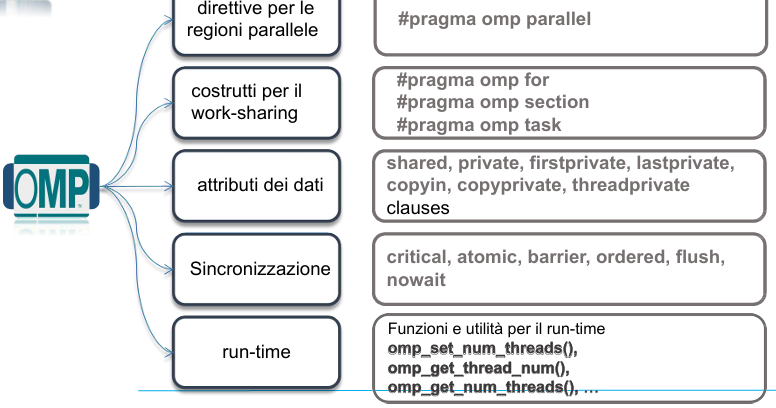
\includegraphics[width=0.6\linewidth]{Images/cap_6/omp_toolbox.png}
\end{figure}

\section{Regioni Parallele}
Come abbiamo visto, OpenMP utilizza il modello fork-join. Il lavoro parallelo si svolge all'interno di \textbf{regioni parallele}, che in C/C++ vengono definite applicando una direttiva a un blocco di codice strutturato.


Quando il compilatore incontra la direttiva \texttt{\#pragma omp parallel}, crea un pool di thread. Ognuno di essi riceve un ID univoco (da $0$ a $N-1$): \textbf{ogni thread riceve un proprio Stack privato e un proprio Instruction Pointer (IP)} separati da quelli del processo padre.

Le direttive in generale in C/C++ sono di questo tipo:
\begin{center}
    \texttt{\#pragma omp <directive> [<clause> [ <clause> [...]]]}
\end{center}

